\chapter{Q08}
\emph{Q8: What is geographical routing? Give one or two examples of
geographical routing protocol and briefly describe the routing mechanism of the
examples.}

\section{Geographical routing}

Transmit package to region r.

Distination in package.

Assume that motes knows their location.

\subsection{Greedy routing}

achieve max progress towards D

- Next hop is the neighbor that gets the packet closest to destination

fails when reaching a ``dead end'' (or void, or local minima)

\subsection{Greedy Perimeter Stateless Routing}

\subsection{Geographic routing without positions}

Virtual Polar Coordinate Space (VPCS)

Choose a root node
Build a tree:

\begin{center}
 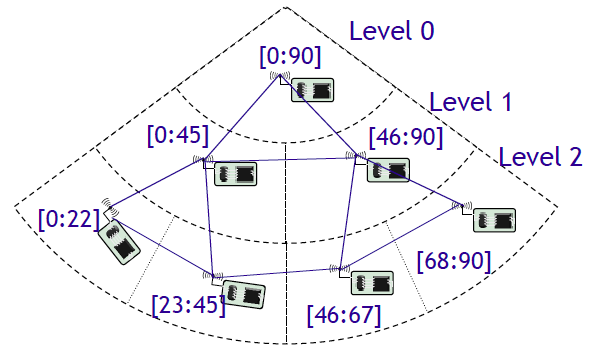
\includegraphics[scale=0.5]{img/Routing-VPCS.png}
\end{center}

\begin{description}
	\item Basic scheme (Naive tree)
	\item Smart tree
	\item Greedy forwarding in polar coordinates.
\end{description}
